\section{Experiments}
\label{sec:exp}

\paragraph{Protocol.} All numbers in this section come from one front-end pass over the 526 benchmark clips in which every variant of \method shares the OCR, tracking and instance estimation, so variants are paired clip by clip; all methods (including the original clips and \steer) are read by the same reader in the same evaluation job (\cref{sec:metrics}). Paired differences are reported with 95\% bootstrap confidence intervals over clips~\cite{efron1994bootstrap} and readability differences with exact McNemar tests~\cite{mcnemar1947}. Forty clips were inspected while developing the selective-editing components (\cref{sec:exp_sel}); \cref{tab:main} reports all clips and, separately, the 486 clips that were never inspected.

\paragraph{Baseline.} \steer~\cite{zeng2026steervte} is the strongest published video text editor; it adds glyph and style conditioning to a frozen VACE-14B backbone~\cite{jiang2025vace} and is trained on one million triplets. We ran the released model on every clip with the hint box as editing mask and the target as text, at the same resolution and length as the input. Its outputs are generated end to end, so they are evaluated as they are.

% generated by paper_numbers.py: Table 1 from r1full (one front-end pass, one evaluation job)
\begin{table*}[t]
\centering
\caption{\textbf{Main results} (526 clips; one front-end pass and one evaluation job for every row). Readability: share of clips whose text the reader transcribes exactly in at least 4 of 5 frames. Fixed / broken: garbled $\to$ correct and correct $\to$ wrong transitions relative to the original as read in the same job; net = fixed $-$ broken. Appearance: glyph-agnostic material distance to the original text (normalised within this run; lower is closer). BG PSNR: outside the dilated text region. Flicker and jitter: motion-compensated, inside the text box (grey levels). The lower block excludes the 40 clips inspected while developing the selective-editing components.}
\label{tab:main}
\setlength{\tabcolsep}{4.5pt}
\resizebox{\linewidth}{!}{%
\begin{tabular}{@{}lccccccccc@{}}
\toprule
 & Readability $\uparrow$ & Fixed $\uparrow$ & Broken $\downarrow$ & Net $\uparrow$ & NED sim.\ $\uparrow$ & Appearance $\downarrow$ & BG PSNR $\uparrow$ & Flicker $\downarrow$ & Jitter $\downarrow$ \\
\midrule
\multicolumn{10}{@{}l}{\emph{All 526 clips}} \\
Original (generated) & 53.8 & -- & -- & -- & 0.820 & -- & -- & 1.98 & 9.18 \\
\steer~\cite{zeng2026steervte} & 84.0 & 165 & \textbf{6} & 159 & 0.946 & \textbf{1.83} & 36.49 & \textbf{1.66} & 8.30 \\
\method & \textbf{91.4} & \textbf{210} & 12 & \textbf{198} & \textbf{0.959} & 2.57 & \textbf{42.52} & 1.79 & \textbf{7.86} \\
\midrule
\multicolumn{10}{@{}l}{\emph{486 clips outside the development set}} \\
Original (generated) & 54.7 & -- & -- & -- & 0.822 & -- & -- & 1.97 & 9.12 \\
\steer~\cite{zeng2026steervte} & 84.4 & 150 & \textbf{6} & 144 & 0.945 & \textbf{1.85} & 36.40 & \textbf{1.65} & 8.24 \\
\method & \textbf{91.2} & \textbf{189} & 12 & \textbf{177} & \textbf{0.958} & 2.60 & \textbf{42.50} & 1.79 & \textbf{7.86} \\
\bottomrule
\end{tabular}}
\end{table*}


\subsection{Main results}
\label{sec:main}
\Cref{tab:main} compares \method with \steer and with the unedited clips. \method makes 91.4\% of the clips readable, 7.4 points more than \steer (69 clips are correct only with \method, 30 only with \steer; McNemar $p=1.1\times10^{-4}$), and turns 212 of the 242 garbled clips into correct ones. It is not free of damage: it breaks 15 of the 284 originally correct clips where \steer breaks 6, so its advantage in net repairs (197 vs.\ 158) is smaller than in repairs alone. The picture is unchanged on the 486 clips outside the development set (91.2\% vs.\ 84.2\%; 175 vs.\ 141 net repairs).

The two methods trade different qualities. \method leaves the background intact---its PSNR outside the text region is 6.4\,dB higher (95\% CI [6.2, 6.7]; higher on 98.1\% of the clips)---and its strokes jitter less (edge jitter 7.85 vs.\ 8.34), because every glyph is placed once on the tracked carrier. \steer's text region flickers less (1.66 vs.\ 1.79) and, above all, its text looks more like the original: its appearance distance is 1.83 against 2.53 for \method. We analyse this gap in \cref{sec:limits}.

\Cref{fig:material} breaks readability down by carrier material. \method is ahead of \steer on six materials and level on wood; the largest gains are on signboards (+15.1 points) and screens (+10.8), where \steer most often keeps the garbled characters. By language, \method reaches 90.2\% on the 295 English and 93.1\% on the 231 Chinese clips (\steer: 84.1\% and 84.0\%). \Cref{fig:qual} shows randomly sampled examples, including a failure of \method (\zh{花店}, glass).

\begin{figure}[t]
\centering
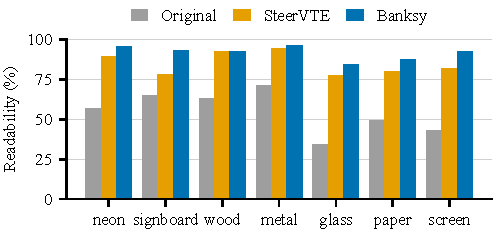
\includegraphics[width=\linewidth]{figs/plots/material_readability.pdf}
\caption{\textbf{Readability by carrier material} (all 526 clips; 54 to 96 clips per material).}
\label{fig:material}
\end{figure}

\begin{figure*}[t]
\centering
\setlength{\tabcolsep}{1.2pt}\renewcommand{\arraystretch}{0.6}
\begin{tabular}{@{}m{0.95cm}cccccc@{}}
&\footnotesize\textbf{Original} & \footnotesize\textbf{SteerVTE} & \footnotesize\textbf{Banksy} & \footnotesize\textbf{Original} & \footnotesize\textbf{SteerVTE} & \footnotesize\textbf{Banksy} \\[2pt]
\scriptsize neon & 
\includegraphics[width=0.146\linewidth]{figs/cells/qual_g001_en_neon_s2_orig.jpg} & 
\includegraphics[width=0.146\linewidth]{figs/cells/qual_g001_en_neon_s2_steervte.jpg} & 
\includegraphics[width=0.146\linewidth]{figs/cells/qual_g001_en_neon_s2_B1.jpg} & 
\includegraphics[width=0.146\linewidth]{figs/cells/qual_g100_zh_neon_s5_orig.jpg} & 
\includegraphics[width=0.146\linewidth]{figs/cells/qual_g100_zh_neon_s5_steervte.jpg} & 
\includegraphics[width=0.146\linewidth]{figs/cells/qual_g100_zh_neon_s5_B1.jpg} \\
&\parbox[t]{0.146\linewidth}{\centering\scriptsize \textcolor{badred}{\ding{55}}\,\texttt{OFFEE SHOP}} & \parbox[t]{0.146\linewidth}{\centering\scriptsize \textcolor{okgreen}{\ding{51}}\,\texttt{COFFEE SHOP}} & \parbox[t]{0.146\linewidth}{\centering\scriptsize \textcolor{okgreen}{\ding{51}}\,\texttt{COFFEE SHOP}} & \parbox[t]{0.146\linewidth}{\centering\scriptsize \textcolor{badred}{\ding{55}}\,\texttt{\zh{公公}}} & \parbox[t]{0.146\linewidth}{\centering\scriptsize \textcolor{okgreen}{\ding{51}}\,\texttt{\zh{公园}}} & \parbox[t]{0.146\linewidth}{\centering\scriptsize \textcolor{badred}{\ding{55}}\,\texttt{\zh{公园}}} \\[3pt]
\scriptsize signboard & 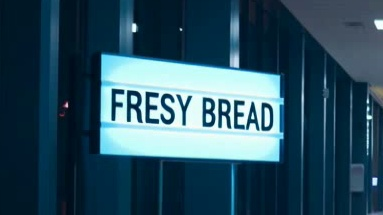
\includegraphics[width=0.146\linewidth]{figs/cells/qual_g008_en_signboard_s4_orig.jpg} & 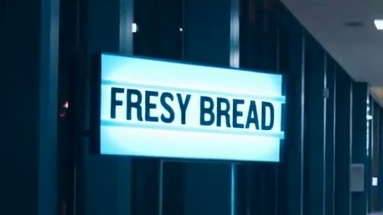
\includegraphics[width=0.146\linewidth]{figs/cells/qual_g008_en_signboard_s4_steervte.jpg} & 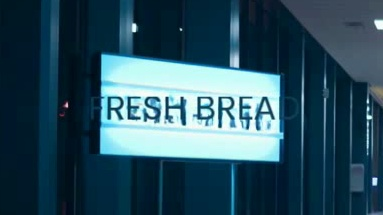
\includegraphics[width=0.146\linewidth]{figs/cells/qual_g008_en_signboard_s4_B1.jpg} & 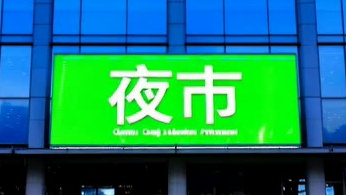
\includegraphics[width=0.146\linewidth]{figs/cells/qual_g085_zh_signboard_s8_orig.jpg} & 
\includegraphics[width=0.146\linewidth]{figs/cells/qual_g085_zh_signboard_s8_steervte.jpg} & 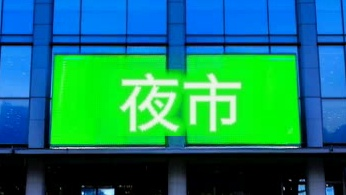
\includegraphics[width=0.146\linewidth]{figs/cells/qual_g085_zh_signboard_s8_B1.jpg} \\
&\parbox[t]{0.146\linewidth}{\centering\scriptsize \textcolor{badred}{\ding{55}}\,\texttt{FRESY BREAD}} & \parbox[t]{0.146\linewidth}{\centering\scriptsize \textcolor{badred}{\ding{55}}\,\texttt{FRESY BREAD}} & \parbox[t]{0.146\linewidth}{\centering\scriptsize \textcolor{okgreen}{\ding{51}}\,\texttt{FRESH BREAD}} & \parbox[t]{0.146\linewidth}{\centering\scriptsize \textcolor{badred}{\ding{55}}\,\texttt{\zh{夜市} Qingdao Night Marke}} & \parbox[t]{0.146\linewidth}{\centering\scriptsize \textcolor{okgreen}{\ding{51}}\,\texttt{\zh{夜市}}} & \parbox[t]{0.146\linewidth}{\centering\scriptsize \textcolor{okgreen}{\ding{51}}\,\texttt{\zh{夜市}}} \\[3pt]
\scriptsize wood & 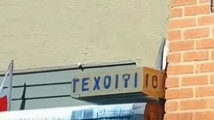
\includegraphics[width=0.146\linewidth]{figs/cells/qual_g014_en_wood_s6_orig.jpg} & 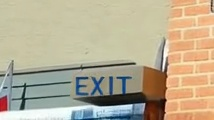
\includegraphics[width=0.146\linewidth]{figs/cells/qual_g014_en_wood_s6_steervte.jpg} & 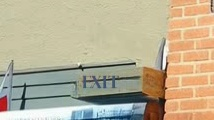
\includegraphics[width=0.146\linewidth]{figs/cells/qual_g014_en_wood_s6_B1.jpg} & 
\includegraphics[width=0.146\linewidth]{figs/cells/qual_g105_zh_wood_s1_orig.jpg} & 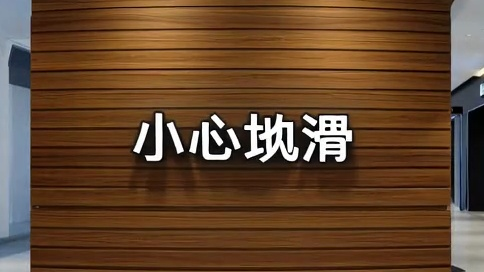
\includegraphics[width=0.146\linewidth]{figs/cells/qual_g105_zh_wood_s1_steervte.jpg} & 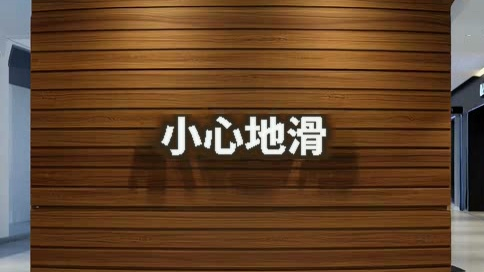
\includegraphics[width=0.146\linewidth]{figs/cells/qual_g105_zh_wood_s1_B1.jpg} \\
&\parbox[t]{0.146\linewidth}{\centering\scriptsize \textcolor{badred}{\ding{55}}\,\texttt{TEXOITYIO}} & \parbox[t]{0.146\linewidth}{\centering\scriptsize \textcolor{okgreen}{\ding{51}}\,\texttt{EXIT}} & \parbox[t]{0.146\linewidth}{\centering\scriptsize \textcolor{okgreen}{\ding{51}}\,\texttt{EXIT}} & \parbox[t]{0.146\linewidth}{\centering\scriptsize \textcolor{badred}{\ding{55}}\,\texttt{\zh{小悒念滑}}} & \parbox[t]{0.146\linewidth}{\centering\scriptsize \textcolor{okgreen}{\ding{51}}\,\texttt{\zh{小心地滑}}} & \parbox[t]{0.146\linewidth}{\centering\scriptsize \textcolor{okgreen}{\ding{51}}\,\texttt{\zh{小心地滑}}} \\[3pt]
\scriptsize metal & 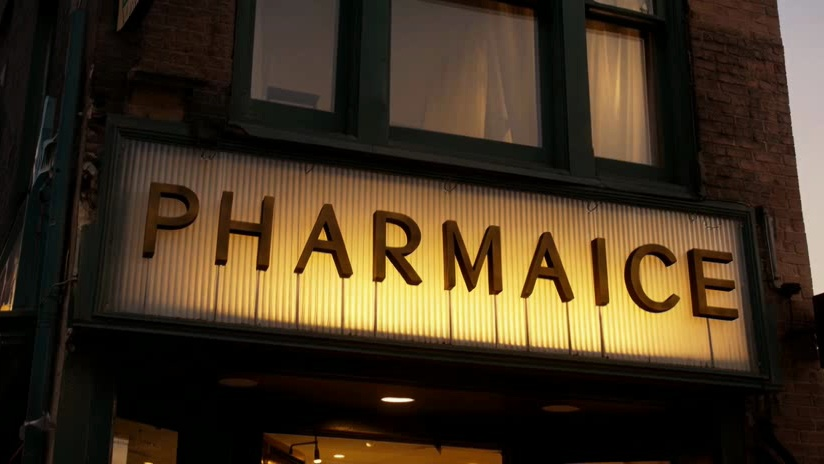
\includegraphics[width=0.146\linewidth]{figs/cells/qual_g024_en_metal_s2_orig.jpg} & 
\includegraphics[width=0.146\linewidth]{figs/cells/qual_g024_en_metal_s2_steervte.jpg} & 
\includegraphics[width=0.146\linewidth]{figs/cells/qual_g024_en_metal_s2_B1.jpg} & 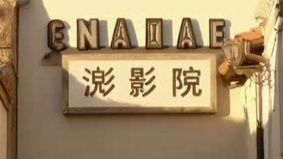
\includegraphics[width=0.146\linewidth]{figs/cells/qual_g089_zh_metal_s3_orig.jpg} & 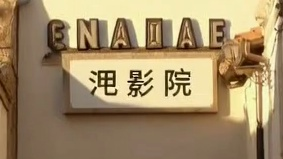
\includegraphics[width=0.146\linewidth]{figs/cells/qual_g089_zh_metal_s3_steervte.jpg} & 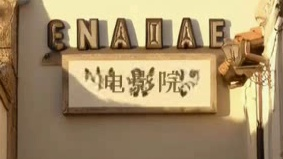
\includegraphics[width=0.146\linewidth]{figs/cells/qual_g089_zh_metal_s3_B1.jpg} \\
&\parbox[t]{0.146\linewidth}{\centering\scriptsize \textcolor{badred}{\ding{55}}\,\texttt{PHARMAICE}} & \parbox[t]{0.146\linewidth}{\centering\scriptsize \textcolor{okgreen}{\ding{51}}\,\texttt{PHARMACY}} & \parbox[t]{0.146\linewidth}{\centering\scriptsize \textcolor{okgreen}{\ding{51}}\,\texttt{PHARMACY}} & \parbox[t]{0.146\linewidth}{\centering\scriptsize \textcolor{badred}{\ding{55}}\,\texttt{\zh{澎影院}}} & \parbox[t]{0.146\linewidth}{\centering\scriptsize \textcolor{badred}{\ding{55}}\,\texttt{\zh{洹影院}}} & \parbox[t]{0.146\linewidth}{\centering\scriptsize \textcolor{okgreen}{\ding{51}}\,\texttt{\zh{电影院}}} \\[3pt]
\scriptsize glass & 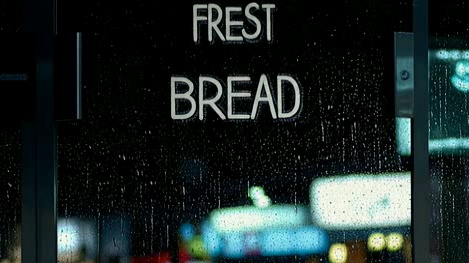
\includegraphics[width=0.146\linewidth]{figs/cells/qual_g007_en_glass_s2_orig.jpg} & 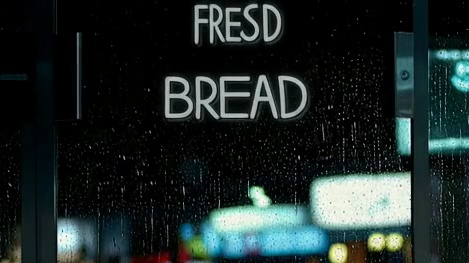
\includegraphics[width=0.146\linewidth]{figs/cells/qual_g007_en_glass_s2_steervte.jpg} & 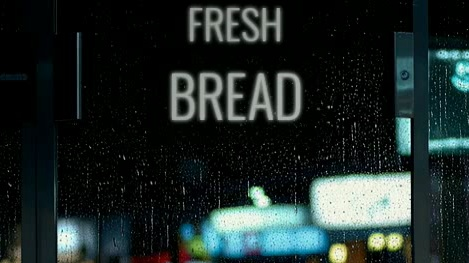
\includegraphics[width=0.146\linewidth]{figs/cells/qual_g007_en_glass_s2_B1.jpg} & 
\includegraphics[width=0.146\linewidth]{figs/cells/qual_g090_zh_glass_s7_orig.jpg} & 
\includegraphics[width=0.146\linewidth]{figs/cells/qual_g090_zh_glass_s7_steervte.jpg} & 
\includegraphics[width=0.146\linewidth]{figs/cells/qual_g090_zh_glass_s7_B1.jpg} \\
&\parbox[t]{0.146\linewidth}{\centering\scriptsize \textcolor{badred}{\ding{55}}\,\texttt{FREST BREAD}} & \parbox[t]{0.146\linewidth}{\centering\scriptsize \textcolor{badred}{\ding{55}}\,\texttt{FRESB BREAD}} & \parbox[t]{0.146\linewidth}{\centering\scriptsize \textcolor{okgreen}{\ding{51}}\,\texttt{FRESH BREAD}} & \parbox[t]{0.146\linewidth}{\centering\scriptsize \textcolor{badred}{\ding{55}}\,\texttt{\cjkimg{cjk_b7d9d7d024} HUAJANGDIAN}} & \parbox[t]{0.146\linewidth}{\centering\scriptsize \textcolor{okgreen}{\ding{51}}\,\texttt{\zh{花店}}} & \parbox[t]{0.146\linewidth}{\centering\scriptsize \textcolor{badred}{\ding{55}}\,\texttt{\zh{南湖公园}}} \\[3pt]
\scriptsize paper & 
\includegraphics[width=0.146\linewidth]{figs/cells/qual_g034_en_paper_s3_orig.jpg} & 
\includegraphics[width=0.146\linewidth]{figs/cells/qual_g034_en_paper_s3_steervte.jpg} & 
\includegraphics[width=0.146\linewidth]{figs/cells/qual_g034_en_paper_s3_B1.jpg} & 
\includegraphics[width=0.146\linewidth]{figs/cells/qual_g096_zh_paper_s0_orig.jpg} & 
\includegraphics[width=0.146\linewidth]{figs/cells/qual_g096_zh_paper_s0_steervte.jpg} & 
\includegraphics[width=0.146\linewidth]{figs/cells/qual_g096_zh_paper_s0_B1.jpg} \\
&\parbox[t]{0.146\linewidth}{\centering\scriptsize \textcolor{badred}{\ding{55}}\,\texttt{SALE}} & \parbox[t]{0.146\linewidth}{\centering\scriptsize \textcolor{badred}{\ding{55}}\,\texttt{SALE}} & \parbox[t]{0.146\linewidth}{\centering\scriptsize \textcolor{okgreen}{\ding{51}}\,\texttt{SALE 50\%}} & \parbox[t]{0.146\linewidth}{\centering\scriptsize \textcolor{badred}{\ding{55}}\,\texttt{\zh{洗衣}}} & \parbox[t]{0.146\linewidth}{\centering\scriptsize \textcolor{okgreen}{\ding{51}}\,\texttt{\zh{洗衣店}}} & \parbox[t]{0.146\linewidth}{\centering\scriptsize \textcolor{okgreen}{\ding{51}}\,\texttt{\zh{洗衣店}}} \\[3pt]
\scriptsize screen & 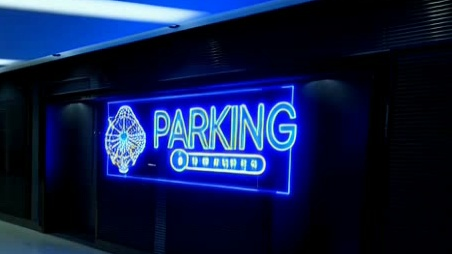
\includegraphics[width=0.146\linewidth]{figs/cells/qual_g029_en_screen_s3_orig.jpg} & 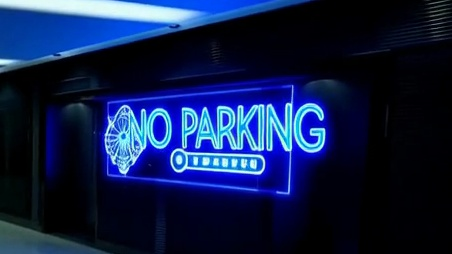
\includegraphics[width=0.146\linewidth]{figs/cells/qual_g029_en_screen_s3_steervte.jpg} & 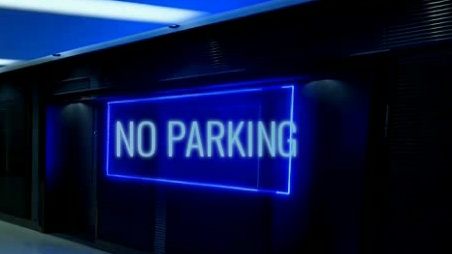
\includegraphics[width=0.146\linewidth]{figs/cells/qual_g029_en_screen_s3_B1.jpg} & 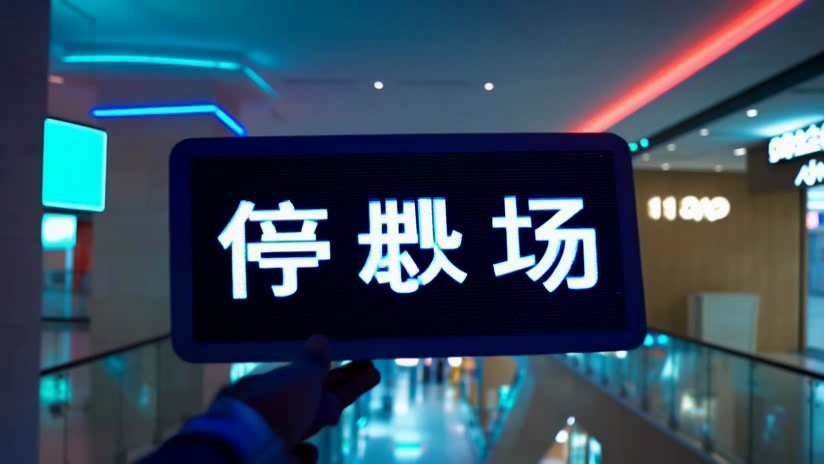
\includegraphics[width=0.146\linewidth]{figs/cells/qual_g078_zh_screen_s4_orig.jpg} & 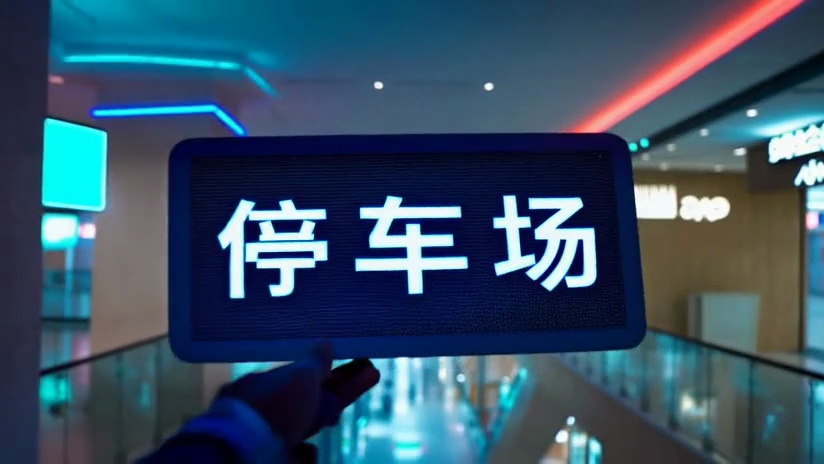
\includegraphics[width=0.146\linewidth]{figs/cells/qual_g078_zh_screen_s4_steervte.jpg} & 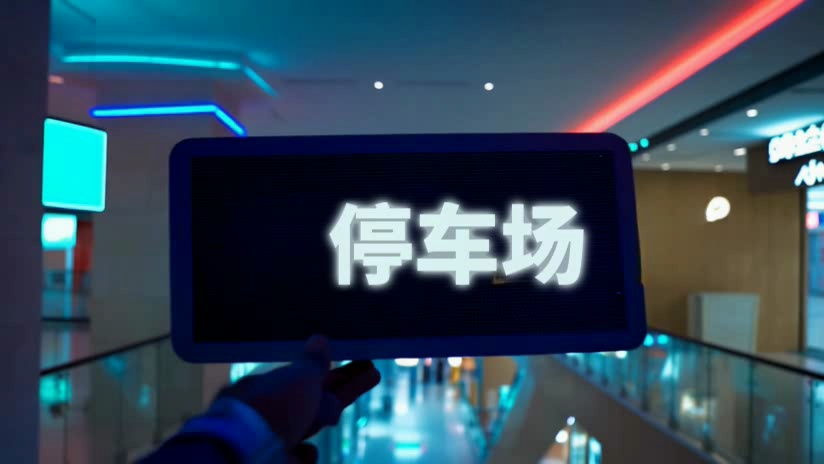
\includegraphics[width=0.146\linewidth]{figs/cells/qual_g078_zh_screen_s4_B1.jpg} \\
&\parbox[t]{0.146\linewidth}{\centering\scriptsize \textcolor{badred}{\ding{55}}\,\texttt{PARKING}} & \parbox[t]{0.146\linewidth}{\centering\scriptsize \textcolor{okgreen}{\ding{51}}\,\texttt{NO PARKING}} & \parbox[t]{0.146\linewidth}{\centering\scriptsize \textcolor{okgreen}{\ding{51}}\,\texttt{NO PARKING}} & \parbox[t]{0.146\linewidth}{\centering\scriptsize \textcolor{badred}{\ding{55}}\,\texttt{\cjkimg{cjk_9107d7aedf}}} & \parbox[t]{0.146\linewidth}{\centering\scriptsize \textcolor{okgreen}{\ding{51}}\,\texttt{\zh{停车场}}} & \parbox[t]{0.146\linewidth}{\centering\scriptsize \textcolor{okgreen}{\ding{51}}\,\texttt{\zh{停车场}}} \\[3pt]
\end{tabular}
\caption{\textbf{Qualitative comparison on randomly sampled clips} (one English and one Chinese clip per material, drawn with a fixed seed among garbled originals outside the development set; not curated). Each cell is the same crop of frame 24; below it, the reader's transcription (\textcolor{okgreen}{\ding{51}}~correct, \textcolor{badred}{\ding{55}}~wrong). SteerVTE produces more natural glyphs but frequently keeps or invents wrong characters; Banksy writes the target but its glyphs often look pasted (see \cref{sec:limits}).}
\label{fig:qual}
\end{figure*}

% Background fidelity: absolute grey-level difference to the original frame (clipped at 24), full frame, frame 24; Banksy = al_r1 B1 outputs.
\begin{figure}[t]
\centering
\setlength{\tabcolsep}{1pt}\renewcommand{\arraystretch}{0.5}
\begin{tabular}{@{}ccc@{}}
\footnotesize Original & \footnotesize $|\,$\steer $-$ original$\,|$ & \footnotesize $|\,$\method $-$ original$\,|$ \\[2pt]
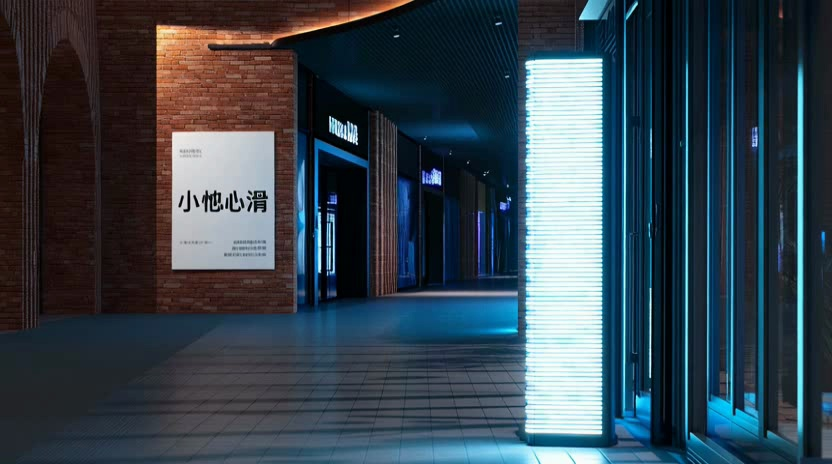
\includegraphics[width=0.325\linewidth]{figs/cells/diff_g106_zh_paper_s6_orig.jpg} &
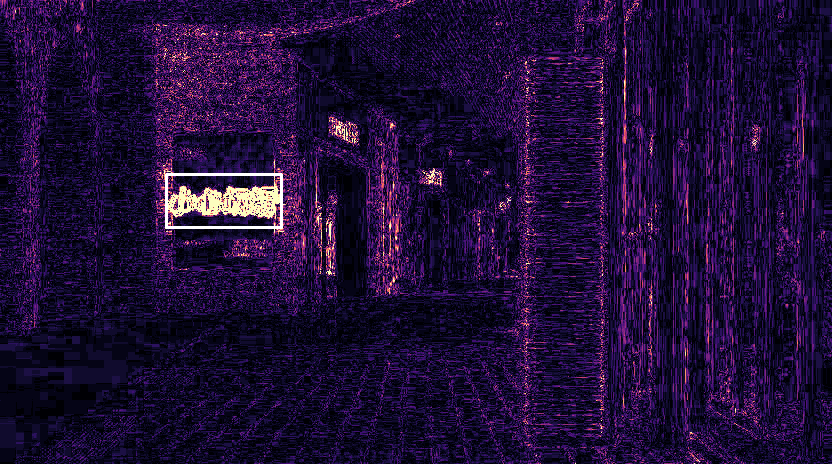
\includegraphics[width=0.325\linewidth]{figs/cells/diff_g106_zh_paper_s6_steervte_diff.png} &

\includegraphics[width=0.325\linewidth]{figs/cells/diff_g106_zh_paper_s6_B1_diff.png} \\
 & \scriptsize outside: 2.58 & \scriptsize outside: 1.74 \\[2pt]
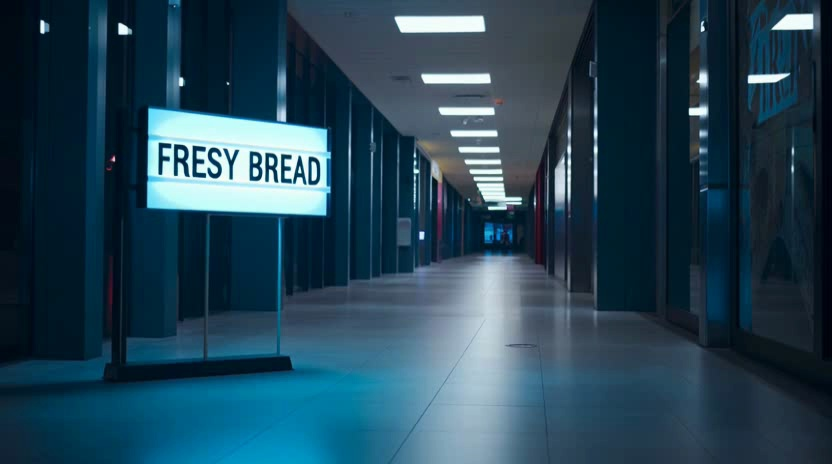
\includegraphics[width=0.325\linewidth]{figs/cells/diff_g008_en_signboard_s4_orig.jpg} &
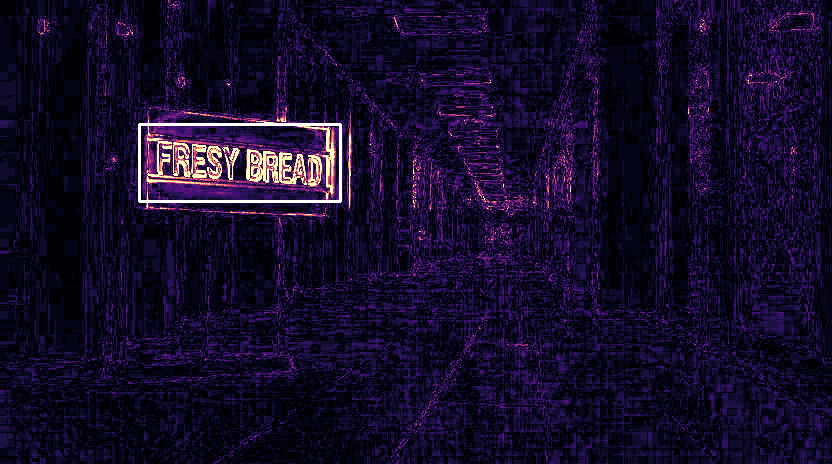
\includegraphics[width=0.325\linewidth]{figs/cells/diff_g008_en_signboard_s4_steervte_diff.png} &

\includegraphics[width=0.325\linewidth]{figs/cells/diff_g008_en_signboard_s4_B1_diff.png} \\
 & \scriptsize outside: 1.70 & \scriptsize outside: 0.95 \\[2pt]
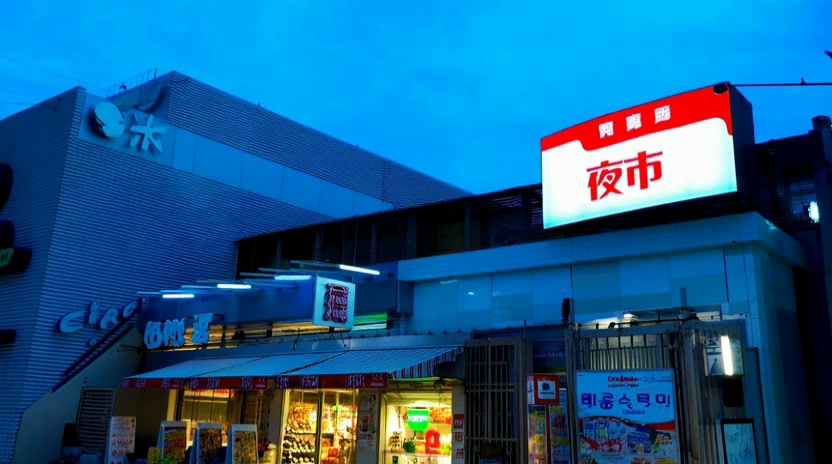
\includegraphics[width=0.325\linewidth]{figs/cells/diff_g085_zh_signboard_s0_orig.jpg} &
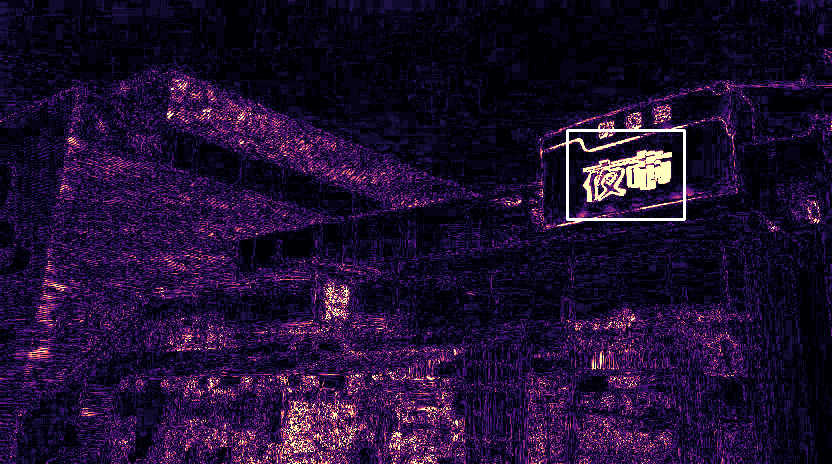
\includegraphics[width=0.325\linewidth]{figs/cells/diff_g085_zh_signboard_s0_steervte_diff.png} &
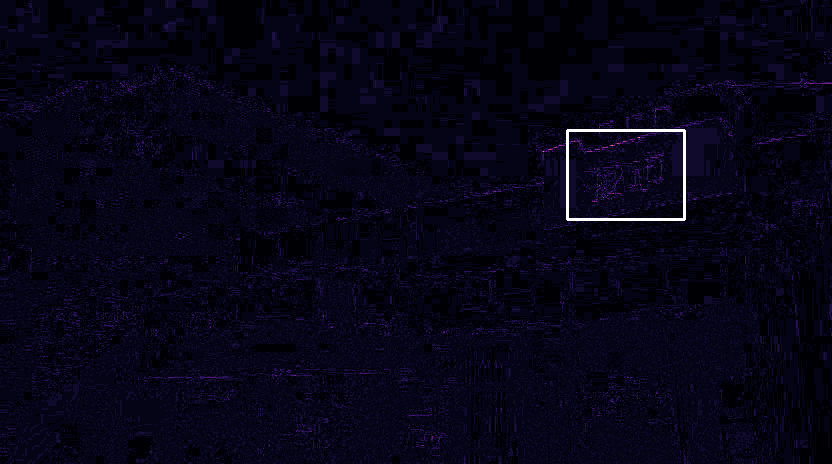
\includegraphics[width=0.325\linewidth]{figs/cells/diff_g085_zh_signboard_s0_B1_diff.png} \\
 & \scriptsize outside: 2.53 & \scriptsize outside: 0.88 (untouched) \\
\end{tabular}
\caption{\textbf{Edit locality.} Absolute grey-level difference to the original frame (clipped at 24; white box: text region). \steer re-renders the whole frame, so residual edges appear everywhere; \method changes only the text region. The numbers give the mean absolute difference outside the dilated text region. \method's residual there (1--2 grey levels, block artefacts of the output codec) is the video re-encoding floor, visible alone in the bottom row, where the preservation gate leaves an already-correct clip untouched while \steer still alters it.}
\label{fig:diff}
\end{figure}


\subsection{Edit locality}
\label{sec:exp_local}
\Cref{fig:diff} visualises where each method changes the video. Because \steer passes the whole clip through its generator, its difference to the original covers the entire frame, including edges of buildings and furniture far from the text; for \method, the difference is confined to the text region, and the residual elsewhere ($\approx$1 grey level) is the re-encoding of the output video. Inside the neighbourhood of the text, we additionally measure the \emph{collateral change}---the change outside both the old and the new glyphs---which is 1.54 grey levels for \method; it cannot be computed for \steer, whose glyph coverage is unknown.

\subsection{The evidence gates}
\label{sec:exp_gates}
\paragraph{Preservation gate.} The gate skips 46 clips, and the reader confirms all 46 as correct (no false skip; the pre-registered limit was 2\%). It restores 2 of the 17 originally correct clips that \method would otherwise break, which is the entire readability difference between the two rows of \cref{tab:main} (2 vs.\ 0 discordant clips, $p=0.5$). Its recall is low by design: it fires on 46 of the 284 clips the reader judges correct (16\%), because the pipeline's OCR rarely reads stylised originals---neon italics, extruded letters, condensed faces---with the required consistency. All 15 originally correct clips that \method breaks are such cases (\cref{sec:failures}).

% Component ablations (earlier front end; experiments T and D, sheets 15-16) and front-end variants (sheet 30), 526 clips.
% Appearance is normalised within each evaluation job, so it is comparable only inside one block.
\begin{table*}[t]
\centering
\begin{minipage}[t]{0.43\linewidth}
\centering
\caption{\textbf{Rendering components} (earlier front end, 526 clips). Top: carrier-anchored temporal components; bottom: style-matched rendering. Appearance is normalised within each block. The box policy used by \method's fallback is T4 + D2.}
\label{tab:components}
\small\setlength{\tabcolsep}{2.4pt}
\resizebox{\linewidth}{!}{%
\begin{tabular}{@{}lcccc@{}}
\toprule
 & Read.\ $\uparrow$ & Flicker $\downarrow$ & Jitter $\downarrow$ & Appear.\ $\downarrow$ \\
\midrule
Original & 53.8 & 1.98 & 9.18 & -- \\
\steer & 83.8 & 1.66 & 8.30 & -- \\
Naive paste (per-frame OCR box) & 87.1 & 3.12 & 11.66 & -- \\
\quad + carrier tracking (T1) & 87.3 & 2.80 & 10.28 & -- \\
\quad + carrier-space erasure (T2) & 88.6 & 2.19 & 9.27 & -- \\
\quad + anchored masks, ink smoothing (T3) & 87.1 & 3.06 & 11.47 & -- \\
\quad + all three (T4) & 89.0 & 1.67 & 7.12 & -- \\
\midrule
\steer & 83.8 & -- & -- & 1.39 \\
Naive paste & 86.9 & -- & -- & 1.89 \\
\quad + font matching (D1) & 89.5 & -- & -- & 1.83 \\
\quad + per-frame ink, shading field (D2) & 89.4 & -- & -- & 1.82 \\
\quad + edge blur and grain (D3) & 87.6 & -- & -- & 2.01 \\
\bottomrule
\end{tabular}}
\end{minipage}\hfill
\begin{minipage}[t]{0.55\linewidth}
\centering
\caption{\textbf{Front-end variants and the localization gate} (526 clips, one evaluation job). W/L: clips correct only with the variant / only with the box policy (McNemar $p$). Residual: share of old ink still visible, relative to the original, on 24 held-out clips.}
\label{tab:frontend}
\small\setlength{\tabcolsep}{2.4pt}
\resizebox{\linewidth}{!}{%
\begin{tabular}{@{}lccccc@{}}
\toprule
 & Read.\ $\uparrow$ & vs.\ box (W/L, $p$) & Jitter $\downarrow$ & Appear.\ $\downarrow$ & Resid.\ $\downarrow$ \\
\midrule
Original & 53.8 & -- & 9.18 & -- & 1.00 \\
\steer & 84.0 & 33/68, $<$.001 & 8.30 & 1.50 & -- \\
Naive paste & 86.7 & 16/37, .005 & 12.53 & 2.38 & -- \\
Box policy (T4+D2) & 90.7 & -- & 7.80 & 2.27 & 0.42 \\
Instance layout, state-machine tracking & 85.2 & 32/61, .003 & 7.68 & 2.50 & 0.21 \\
Instance layout, carrier tracking & 86.9 & 34/54, .042 & 7.68 & 2.44 & -- \\
\quad + localization gate (\method front end) & 91.1 & 27/25, .89 & 7.66 & 2.33 & 0.23 \\
\bottomrule
\end{tabular}}
\end{minipage}
\end{table*}


\paragraph{Carrier anchoring and style-matched rendering.} \Cref{tab:components} ablates the rendering components on an earlier front end. Pasting the target into the per-frame OCR box makes the text readable but nearly doubles flicker relative to the original clip (3.12 vs.\ 1.98), because OCR boxes jitter from frame to frame. Anchoring everything on the tracked carrier removes most of it: carrier-space erasure contributes most ($-0.93$), tracking $-0.32$ and anchored masks with ink smoothing $-0.05$, and the three together reduce flicker by 1.45, more than the sum of their parts, to the level of \steer (1.67 vs.\ 1.66) while lowering jitter well below it (7.12 vs.\ 8.30). Readability does not suffer (89.0 vs.\ 87.1, $p=0.064$). Matching the font to the old strokes adds 2.6 points of readability (D1; $p=0.044$) once candidates are rendered in the layout of the original---an earlier version compared single-line candidates with two-line originals and systematically picked the thinnest faces. Per-frame ink and a shading field (D2) bring the appearance closest among the rendered variants; imitating edge blur and grain (D3) makes text both less readable and less similar, and was dropped. T4 + D2 constitutes the \emph{box policy}, the fallback of \method.

\paragraph{The localization gate.} Laying the text out on the old glyph instance should look more faithful than filling a box, and on held-out clips it does: it leaves half as much of the old ink visible (residual 0.21 vs.\ 0.42 of the original). On all 526 clips, however, the first instance-aligned front end was 5.5 points \emph{less} readable than the box policy (85.2 vs.\ 90.7; \cref{tab:frontend}). Size and colour were not the cause---forcing the box policy's colour pipeline or a minimum letter height left the gap unchanged (supplement)---but its confidence-based tracking state machine was: replacing it by carrier tracking recovers most of the gap on the clips where an instance is found (90.8 vs.\ 91.3), and the remaining clips are those where the instance estimate itself is unreliable. The localization gate routes exactly these clips to the box policy, which yields a front end that is as readable as the box policy (91.1 vs.\ 90.7; 27 vs.\ 25 discordant clips) while keeping the instance path's lower residual (0.23) and lowest jitter (7.66). Two re-readings of the same outputs differ by about one point (90.3 vs.\ 91.3 in a second job), so we claim parity with the box policy, not superiority. A subset of 100 clips had suggested a gain of one point for an earlier gated variant (95 vs.\ 94) that did not replicate on the full set (88.4 vs.\ 91.3)---a reminder that subset gates are optimistic.


\subsection{Source appearance transport}
\label{sec:exp_sat}
% SAT v1 paired results on the 53 clips where the appearance gate enabled it (full 526-clip pass, sheet 33). Paste only = Banksy front end without SAT.
\begin{table}[t]
\centering
\caption{\textbf{SAT on the clips where the appearance gate enables it} (53 of 526; paired, same front-end pass). $\Delta$: SAT $-$ paste only, with 95\% bootstrap CI.}
\label{tab:sat}
\small\setlength{\tabcolsep}{3pt}
\begin{tabular}{@{}lccc@{}}
\toprule
 & Paste only & + SAT & $\Delta$ [95\% CI] \\
\midrule
Readability (\%) & 98.1 & 100 & +1 clip \\
Appearance $\downarrow$ & 2.97 & 1.95 & $-1.02$ [$-1.70$, $-0.48$] \\
Flicker $\downarrow$ & 2.25 & 2.40 & $+0.15$, $p<0.001$ \\
Jitter $\downarrow$ & 8.62 & 9.42 & $+0.81$, $p=0.001$ \\
BG PSNR (dB) & 43.01 & 43.02 & n.s. \\
\bottomrule
\end{tabular}
\end{table}

% SAT: Original / paste only / + SAT (frame 24, tight crops) and the blind human study (53 SAT-enabled clips, 4 raters).
\begin{figure}[t]
\centering
\setlength{\tabcolsep}{1pt}\renewcommand{\arraystretch}{0.5}
\begin{tabular}{@{}m{1.15cm}ccc@{}}
 & \footnotesize Original & \footnotesize Paste only & \footnotesize + SAT \\[2pt]
\scriptsize \str{PHARMACY} & 
\includegraphics[width=0.265\linewidth]{figs/cells/sat_g026_en_signboard_s5_orig.jpg} & 
\includegraphics[width=0.265\linewidth]{figs/cells/sat_g026_en_signboard_s5_paste.jpg} & 
\includegraphics[width=0.265\linewidth]{figs/cells/sat_g026_en_signboard_s5_sat.jpg} \\
\scriptsize \str{CINEMA} & 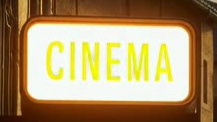
\includegraphics[width=0.265\linewidth]{figs/cells/sat_g017_en_signboard_s1_orig.jpg} & 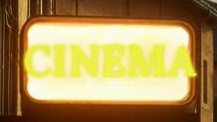
\includegraphics[width=0.265\linewidth]{figs/cells/sat_g017_en_signboard_s1_paste.jpg} & 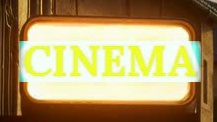
\includegraphics[width=0.265\linewidth]{figs/cells/sat_g017_en_signboard_s1_sat.jpg} \\
\scriptsize \zh{水果店} & 
\includegraphics[width=0.265\linewidth]{figs/cells/sat_g116_zh_screen_s8_orig.jpg} & 
\includegraphics[width=0.265\linewidth]{figs/cells/sat_g116_zh_screen_s8_paste.jpg} & 
\includegraphics[width=0.265\linewidth]{figs/cells/sat_g116_zh_screen_s8_sat.jpg} \\
\scriptsize \zh{营业中}\newline\textcolor{badred}{\tiny failure} & 
\includegraphics[width=0.265\linewidth]{figs/cells/sat_g110_zh_neon_s4_orig.jpg} & 
\includegraphics[width=0.265\linewidth]{figs/cells/sat_g110_zh_neon_s4_paste.jpg} & 
\includegraphics[width=0.265\linewidth]{figs/cells/sat_g110_zh_neon_s4_sat.jpg} \\
\end{tabular}\\[3pt]
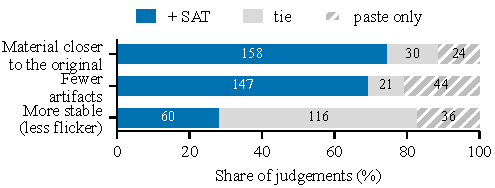
\includegraphics[width=\linewidth]{figs/plots/sat_human.pdf}
\caption{\textbf{Source appearance transport.} Top: SAT carries glow and material of the old glyphs to the new ones (rows 1--3: clips that raters judged better with SAT on both material and artifacts; row 4: a neon clip that all raters judged to have more artifacts with SAT). Bottom: blind pairwise study on all 53 SAT-enabled clips (4 raters, 212 judgements per question; \cref{sec:exp_sat}).}
\label{fig:sat}
\end{figure}


\paragraph{Where the gate enables SAT.} In the pass analysed here, the appearance gate enables SAT on 53 of the 526 clips (in the run of \cref{tab:main}, on \rSatOn): 23 of 93 neon clips, 11 of 65 screens, 9 of 86 signboards, 8 of 56 metal and 2 of 54 wooden signs, and none on glass or paper. Most rejections are clips without an accepted instance (203), followed by non-emissive text (133), no cross-validated gain (104) and gain in only one direction (33). Every enabled clip has a cross-validated error ratio below 0.75 in both directions, and the 15 rejected clips closest to the threshold lie between 0.756 and 0.795.

\paragraph{Effect.} On the enabled clips (\cref{tab:sat}), SAT reduces the appearance distance by a third ($-1.02$; better on 42 of 53 clips) for every material---screens 3.02$\to$1.33, neon 3.03$\to$2.02, wood 4.12$\to$2.21---without hurting readability or the background. It costs temporal stability: flicker rises by 0.15 and jitter by 0.81, because the transported appearance follows a per-frame distance field. On the full benchmark the readability is unchanged (90.5 vs.\ 90.3\%).

\paragraph{Human judgement.} Because the appearance distance is only a proxy, we ran a blind study on all 53 enabled clips (\cref{fig:sat}): raters saw the original between the paste-only and the SAT version in random order and answered three separate questions. Of five raters, one gave the same side on all three questions for 98\% of the clips (including the flicker question, which asks which version is worse) and was excluded by a rule (identical answers on at least 80\% of the clips) that we fixed only after seeing the data; we therefore also report the material question with all five raters. With four raters (212 judgements per question), SAT was judged closer to the original material in 158 cases against 24 (30 ties; win rate 0.87, 95\% CI [0.77, 0.94] by bootstrap over raters and clips; 48 vs.\ 3 clips by majority), and as having fewer artifacts in 147 against 44 (0.77 [0.66, 0.87]); with five raters the material win rate is 0.84 [0.74, 0.92]. Agreement is moderate (Gwet's AC1~\cite{gwet2008ac1} 0.51 for material, 0.61 for artifacts), and the left/right position had no effect after balancing (53\% left, $p=0.27$). The measured flicker increase was not perceived: 55\% of the flicker answers are ties, the remaining answers follow the material answer (a halo effect), and they correlate negatively with the measured flicker change ($\rho=-0.34$). The appearance distance agrees with the material votes only weakly ($\rho=0.28$, $p=0.049$) and not with the artifact votes, so it cannot replace human judgement.

\paragraph{Failures and their cause.} Raters judged six clips to have clearly more artifacts with SAT, four of them neon (\cref{fig:sat}, last row): a bright rectangular plate behind the new letters. A first hypothesis---that the new glyphs reach distances never observed on the old ones---was rejected (the share of unobserved distances is at most 2.3\%), and tapering the operator to identity at the edge of its support had no effect. The plates coincide instead with the canvas on which the new glyphs' distance field is computed: the canvas leaves only 0.04--0.21 letter heights of margin, so the halo, which should extend to 0.6, is cut at the canvas border. With an untruncated distance field the straight edges disappear in our diagnosis, and computing the distance field on a padded canvas reduces flicker by 0.08 and jitter by 0.37 (both better on 47 of 53 clips, $p<0.001$) with no significant change in appearance---about half of SAT's flicker cost and 40\% of its jitter cost. Because these 53 clips were used to diagnose the failure, the padded version is not part of the evaluated \method and requires validation on unseen clips.


\subsection{Selective, structure-preserving editing}
\label{sec:exp_sel}
% generated by make_tab_selective.py from align/sel2/ev1 (one evaluation job for every row)
\begin{table*}[t]
\centering
\caption{\textbf{Selective, structure-preserving editing} (pre-registered; 526 clips; one front-end pass, in which the 99 two-row clips were re-run after a compositing fix, and one evaluation run for every row: all rows read together, every metric computed over all rows at once). B0 is \method without the preservation gate; each component is added to B0 separately and then all three together (B4). Collateral: change outside the old and new glyphs in the text neighbourhood. The verdict applies the pre-registered criteria; development clips are excluded in the right block. The B1 of this pass and the \method of \cref{tab:main} are the same configuration in two independent front-end passes and evaluation runs.}
\label{tab:selective}
\resizebox{\linewidth}{!}{%
\begin{tabular}{@{}lccccccccc|ccc@{}}
\toprule
 & \multicolumn{9}{c|}{All 526 clips} & \multicolumn{3}{c}{486 clips (no development clips)} \\
 & Read.\ $\uparrow$ & Fixed & Broken & Net & Appear.\ $\downarrow$ & BG PSNR & Collateral $\downarrow$ & Flicker & Verdict & Read.\ $\uparrow$ & Net & Collateral $\Delta$ vs.\ B0 \\
\midrule
B0: \method w/o preservation gate & 91.3 & 214 & 16 & 198 & 2.52 & 42.97 & 1.55 & 1.76 & -- & 91.2 & 178 & -- \\
B1: + preservation gate (= \method) & \textbf{91.6} & 214 & \textbf{14} & \textbf{200} & 2.39 & 42.97 & 1.52 & 1.79 & adopted & \textbf{91.4} & \textbf{179} & $-0.031$ [$-0.06$, $-0.01$] \\
B2: + glyph-only erasure & 83.7 & 181 & 23 & 158 & 2.43 & 43.06 & 1.46 & 1.79 & rejected & 84.4 & 145 & $-0.036$ [$-0.09$, $+0.03$] \\
B3: + carrier-fit check & 88.8 & 200 & 15 & 185 & 2.39 & 42.95 & 1.54 & 1.77 & rejected & 88.9 & 167 & $-0.004$ [$-0.01$, $-0.00$] \\
B4: all three & 82.9 & 173 & 19 & 154 & \textbf{2.21} & 43.05 & \textbf{1.43} & 1.82 & rejected & 83.3 & 140 & $-0.062$ [$-0.12$, $+0.01$] \\
\bottomrule
\end{tabular}}
\end{table*}


Inspecting the outputs of the first full evaluation, we found that the most frequent problem of \method was not that its glyphs lacked material but that it changed things it should not have: already-correct text, sign frames, and the structure around the letters. We therefore tested three components that make editing more selective, each added to B0 (\method without the preservation gate) on its own, with acceptance criteria fixed before the run (supplement): the preservation gate of \cref{sec:pres} (B1), \emph{glyph-only erasure} (B2), and a \emph{carrier-fit check} (B3).

\paragraph{Glyph-only erasure (B2).} Instead of inpainting the whole letter band, B2 erases only the old glyphs and their own glow, estimated with a mixture model of carrier, ink and halo colours, and protects sign frames, long bars and the boxes of other text. It is active on the 325 clips with an accepted instance---in 117 of them it falls back to band erasure minus the protected structures, because the surroundings themselves look like strokes (\eg neon stripes)---and its erased area is a median 0.64 of the band area. \emph{Pre-registered criterion}: collateral change decreases ($p<0.05$) and readability drops by at most one point.

\paragraph{Carrier-fit check (B3).} B3 estimates the extent of the carrier from colour, lightness and texture boundaries and declares a clip \emph{layout-infeasible} if the target, at the character density of the source, would have to shrink below 0.7 of the source height to fit; such clips are left unedited and counted as failures. \emph{Criterion}: the infeasible flags are confirmed by manual inspection.

\paragraph{Results.} \Cref{tab:selective} reports all variants from one front-end pass (with the 99 two-row clips re-run after a compositing fix that affects all variants alike). The preservation gate meets its criteria (no false skip; two fewer broken clips; readability not lower) and is adopted, which makes B1 the \method of \cref{tab:main}. Glyph-only erasure reduces collateral change on all clips ($-0.090$, 95\% CI $[-0.17,-0.02]$, $p=0.017$) but not significantly once the development clips are removed ($p=0.23$), and it costs 7.3 points of readability: the instance ink mask is not a complete glyph mask, so parts of the old strokes survive next to the new ones, and OCR boxes of the garbled text itself were sometimes protected as ``other text''. A second version that completes the old glyphs by colour still left remnants in three of nine diagnosed clips, which suggests that this component needs a learned stroke segmentation. Of the 24 clips flagged infeasible by the carrier-fit check, manual inspection confirmed 5, was undecided on 3 and rejected 16 (OCR missed letters of the source, or two-row signs were treated as one row), so B3 is rejected as well; a stricter version that only flags clips whose source stably shows a whole-word part of the target behaved correctly on the diagnosed clips but has not been run at scale. All three together (B4) inherit B2's readability loss. A blind study comparing B1 with \steer (60 clips) and B2 with B0 (28 clips) on naturalness and on damage to non-target content is in progress \pending{(results pending)}.


\subsection{Does a learned refiner help?}
\label{sec:exp_refiner}
% Learned refiner on the 526 clips, all rows read in one evaluation job (workbook sheet 31, complete version).
% W/L vs the same front end without the refiner. Appearance normalised within this job.
\begin{table}[t]
\centering
\caption{\textbf{Does a learned refiner help?} The 1.3B bridge-flow refiner applied on top of \method's front end (paste only) and of the box policy, with and without the carrier-anchored attention bias ($\lambda=2$). 526 clips, one evaluation job; W/L against the same front end without the refiner. Boundary jump: change at the refiner's 17-frame chunk seams relative to other frame pairs (1 = no seam).}
\label{tab:refiner}
\resizebox{\linewidth}{!}{%
\begin{tabular}{@{}lcccccc@{}}
\toprule
 & Read.\ $\uparrow$ & W/L & Flicker $\downarrow$ & Jitter $\downarrow$ & B.\ jump $\downarrow$ & Appear.\ $\downarrow$ \\
\midrule
\steer & 84.2 & -- & 1.66 & 8.34 & 0.93 & 1.58 \\
\midrule
\method front end (paste only) & 91.3 & -- & 1.77 & 7.69 & 0.84 & 2.49 \\
\quad + refiner & 87.8 & 3/21 & 1.96 & 8.22 & 2.26 & 2.45 \\
\quad + refiner + attention bias & 88.6 & 3/17 & 2.00 & 8.41 & 2.06 & 2.33 \\
\midrule
Box policy (paste only) & 91.4 & -- & 1.77 & 7.83 & 0.84 & 2.35 \\
\quad + refiner & 87.6 & 2/22 & 1.99 & 8.46 & 2.31 & 2.31 \\
\quad + refiner + attention bias & 88.4 & 3/19 & 2.03 & 8.68 & 2.10 & 2.24 \\
\bottomrule
\end{tabular}}
\end{table}


Rendered glyphs look pasted, so the obvious remedy is to let a generative model harmonise them with the scene while keeping their shapes. We invested heavily in this route before settling on the training-free pipeline, and report it in full because its outcome shapes our design.

\paragraph{Refiner.} The refiner is a video diffusion transformer initialised from Wan2.1-T2V-1.3B~\cite{wan2025wan} that takes the pasted clip as extra input channels (zero-initialised) and is trained as a flow-matching bridge~\cite{lipman2023flowmatching,liu2023rectifiedflow} from the paste to the target; inference starts from the paste, in the spirit of SDEdit~\cite{meng2022sdedit}, and takes 30 Euler steps on 17-frame chunks of $384\times384$ crops. A glyph loss compares Sobel edges of the decoded prediction with the target inside a band around the glyph (weighted by the signed distance to the glyph boundary). Training pairs come from three sources: a Blender data factory with six carrier surfaces and passing occluders, which renders every sample twice (lit composite and flat paste); 562 real pairs obtained by erasing correct text from generated clips and re-pasting it; and up to 1.15 million image pairs built the same way from AnyWord-3M (63\% LAION, 31\% Wukong, 6\% street scenes). All refiners were trained on H100-class GPUs (GH200/H200) for 20k steps.

\paragraph{More data is not the lever.} On a 296-clip garbled subset, refiners trained with 0, 10k, 100k and 1M image pairs reach 78.4, 75.3, 76.4 and 76.4\% readability, all below the paste they start from (80.7\%), and their appearance does not improve with data (supplement). A diagnostic on 1{,}500 held-out pairs explains why: on the very task they were trained for---turning the paste back into the original---all of them move \emph{away} from the original, they do not even memorise pairs seen twelve times, and they fail to learn a systematic difference (originals have thicker strokes than our pastes in 60\% of the pairs). The supervision was inconsistent: the paste uses our font, the target uses the generator's, and the glyph loss, which dominates the objective, effectively teaches the model to erase our strokes. Making the supervision glyph-consistent---pasting the original's own ink mask instead of our font---is the first recipe that moves toward the original on held-out pairs and it cuts the image-domain readability loss from 26 to 4 points, with appearance better than the paste. On videos, however, it still does not exceed the paste (best variant: 79.7 vs.\ 80.7\%).

\paragraph{System-level effect.} \Cref{tab:refiner} applies the best refiner to the full benchmark. On top of \method's front end it costs 3.5 points of readability (21 clips broken against 3 repaired; $p<0.001$), increases flicker and jitter, and introduces seams at its chunk boundaries (boundary jump 2.26 vs.\ 0.84), while the appearance distance does not change significantly ($-0.035$, 95\% CI $[-0.21, 0.19]$). A training-free attention bias that ties tokens to their carrier trajectory, in the spirit of flow-guided attention~\cite{cong2024flatten,geyer2024tokenflow}, was selected on 50 clips with an earlier refiner (boundary jump $-16\%$ there) and reduces the seams by 9\% on the full set (2.06 vs.\ 2.26; better on 364 of 526 clips), but it slightly increases flicker within chunks and leaves the readability loss in place. We therefore keep the refiner out of \method. The negative result is specific to our scale---1.3B parameters and at most a few hundred real video pairs, against a 14B backbone and a million training triplets for \steer---but it is consistent: at this scale, a learned harmoniser trades the guarantee that motivates rendering for an appearance gain we could not measure.


\subsection{External benchmarks}
\label{sec:exp_external}
Both external evaluations below were run with the earlier box-policy front end (\cref{tab:components}); re-running them with the final pipeline is pending, and we report them as they are.

\paragraph{Editing correct text (VTE-Bench).} On the 100 real clips of \steer's own benchmark~\cite{zeng2026steervte}, where correct text must be changed into a different string, \steer reaches 92\% readability and our earlier pipeline 82\% (8 vs.\ 18 discordant clips, $p=0.076$; a second reader, EasyOCR, gives 49\% vs.\ 44\%). Editing differs from repair: the source text is valid and must be removed entirely, which is the regime that generative editors are trained for and in which our gates provide no advantage. We include the result to delimit our claims.

\paragraph{Commercial video models (VidScribe).} VidScribe~\cite{vidscribe2026} releases the outputs of seven commercial video models for video-to-video text editing. On the 44 of its 93 clips that have a localisable text region, our earlier pipeline reaches 29.5\% (naive paste) and 27.3\% (box policy) readability, ahead of the strongest commercial model (minimax-h3, 18.2\%) and wan-3.0 (15.9\%), although not significantly (box policy vs.\ minimax-h3: 6 vs.\ 2 discordant clips, $p=0.29$); against the other five models (0--13.6\%) the box policy is significantly better ($p\le0.031$). Commercial models regenerate the whole clip and lower the PSNR outside the text region to 19.8--27.9\,dB, against 37.6--37.9\,dB for our outputs. Absolute readability is low for every method because most VidScribe targets are long phrases.

